% Første linje er dokumentklassen. Brug *altid* memoir!
\documentclass[a4paper,oneside,article]{memoir}

% Herunder indlæses forskellige pakker
\usepackage[utf8]{inputenc}  % Korrekt håndtering af æ, ø og å
\usepackage[T1]{fontenc}  % Korrekt håndtering af æ, ø og å
\usepackage{microtype}  % Typografisk magi! Giver bl.a. pænere orddeling
\usepackage{graphicx}  % Gør det muligt at indsætte billeder
\usepackage{amsmath}  % Giver adgang til uundværlige matematikting
\usepackage{mathtools}  % Retter ting i ams og giver ekstra muligheder
\usepackage[danish]{babel}  % Danske betegnelser og orddeling
\usepackage{lmodern}
\usepackage{alphabeta}
\usepackage{float} %Mere kontrol over billede-placering
\renewcommand{\danishhyphenmins}{22}  % Bedre dansk orddeling
\usepackage{siunitx} % Sientific notation for forskellige ting, med en regel om at den skal bruge cdot istedet for times. 
\sisetup{inter-unit-product = \cdot, 
        exponent-product=\cdot}
\usepackage{derivative} % Til at skrive differentialligninger 
\usepackage{xcolor} % For at få flere tekst farver 
\usepackage[colorlinks=true]{hyperref} % For at få refrences man kan trykke på, slet [] hvis man vil have kasser i stedet for farvet tekst.
\usepackage{pdfpages} % Til at indsætte andre pdf'er
\usepackage{subfig} % For at have to billeder ved siden af hinanden
\usepackage{unicode-math}


% Pænere toc indents 
\usepackage{tocloft}
\cftsetindents{section}{1em}{2em}
\cftsetindents{subsection}{4em}{0em}


% Indholdet i dit dokument starter her!
\begin{document}
\author{Mikkel Moth Billing \\ 202307989}
\title{Nuclear and Particle Physics}
\date{\today}
%\maketitle   % Indsætter overskriften
% Table of Contents indstillinger
\setcounter{tocdepth}{2}
\setcounter{secnumdepth}{1}
\hypersetup{linkcolor=black} % Laver tableofcontents sort.  
\tableofcontents %Indsætter ToC
\hypersetup{linkcolor=red} % og så alle andre hyperrefs røde. 

% Custom Commands
\newcommand{\ti}[1]{\cdot 10^{#1}} % Let: gange 10^x
\newcommand{\e}[1]{\emph{e}^{#1}} % Pænere e^x
\newcommand{\vm}[2]{\begin{pmatrix} #1 \\ #2 \end{pmatrix}}
\newcommand{\mat}[1]{\begin{pmatrix} #1 \end{pmatrix}}
\newcommand{\h}{\hbar}
\renewcommand{\v}[1]{\mathbfit{#1}}
\newcommand{\ep}{\epsilon_0}
\newcommand{\M}{\br[5]{\mathscr{M}}^2}

% Atomic Numbers 
\newcommand{\atom}[3]{\!^{#2}_{#3}\text{#1}}

% Lette paranteser 
\newcommand{\br}[2][1]{%
    \ifcase#1
    \or \left( #2 \right) %1 eller ingenting
    \or \left[ #2 \right] %2
    \or \left\langle #2 \right\rangle %3
    \or \left\{ #2 \right\} %4
    \or \left| #2 \right| %5
    \fi
}

% Braket notation
\newcommand{\hv}[2][]{%
    \if\relax\detokenize{#1}\relax
        |#2\rangle%
    \else
        \if\relax\detokenize{#2}\relax
            \langle #1|%
        \else
            \langle #1|#2\rangle%
        \fi
    \fi
}

% Til at sætter bileder ind i store dokumenter
\newcommand{\bil}[1]{
\begin{figure}[H]
    \centering
    \includegraphics[width=0.75\linewidth]{Billeder/#1.png}
    \caption{}
    \label{fig:#1}
\end{figure}
}

% Til at sætte pdf'er ind i store dokumenter (kun pdf'er på mere end 1 sider)
\newcommand{\pdf}[4]{
\includepdf[pages=#3,scale=.85,pagecommand={\subsection{#2 - \ref{ch:opg}}  \label{asc:#2}}]{pdf/#1.pdf}
\includepdf[pages=\the\numexpr 1 + #3\relax-#4, scale=.85]{pdf/#1.pdf}
}

% Til at Give equation numre 
\newcommand{\eq}[1]{\label{eq:#1}\tag{#1}}

% Lav ny pagestyle (kun odd fordi enkeltsidet)
\makepagestyle{Title}
\pagestyle{Title}
%\makeoddhead{Title}{\footnotesize\color{gray}{\theauthor}}{}{\textcolor{gray}{\thedate}}
\makeoddfoot{Title}{}{\footnotesize\color{gray}{\thepage{} / \thelastpage}}{}
% Også fod på siden med \maketitle
\makeoddfoot{plain}{}{\footnotesize\color{gray}{\thepage{} / \thelastpage}}{}
\newpage

%Skriv
\chapter{Fundamental Particles}
\begin{figure}[H]
    \centerline{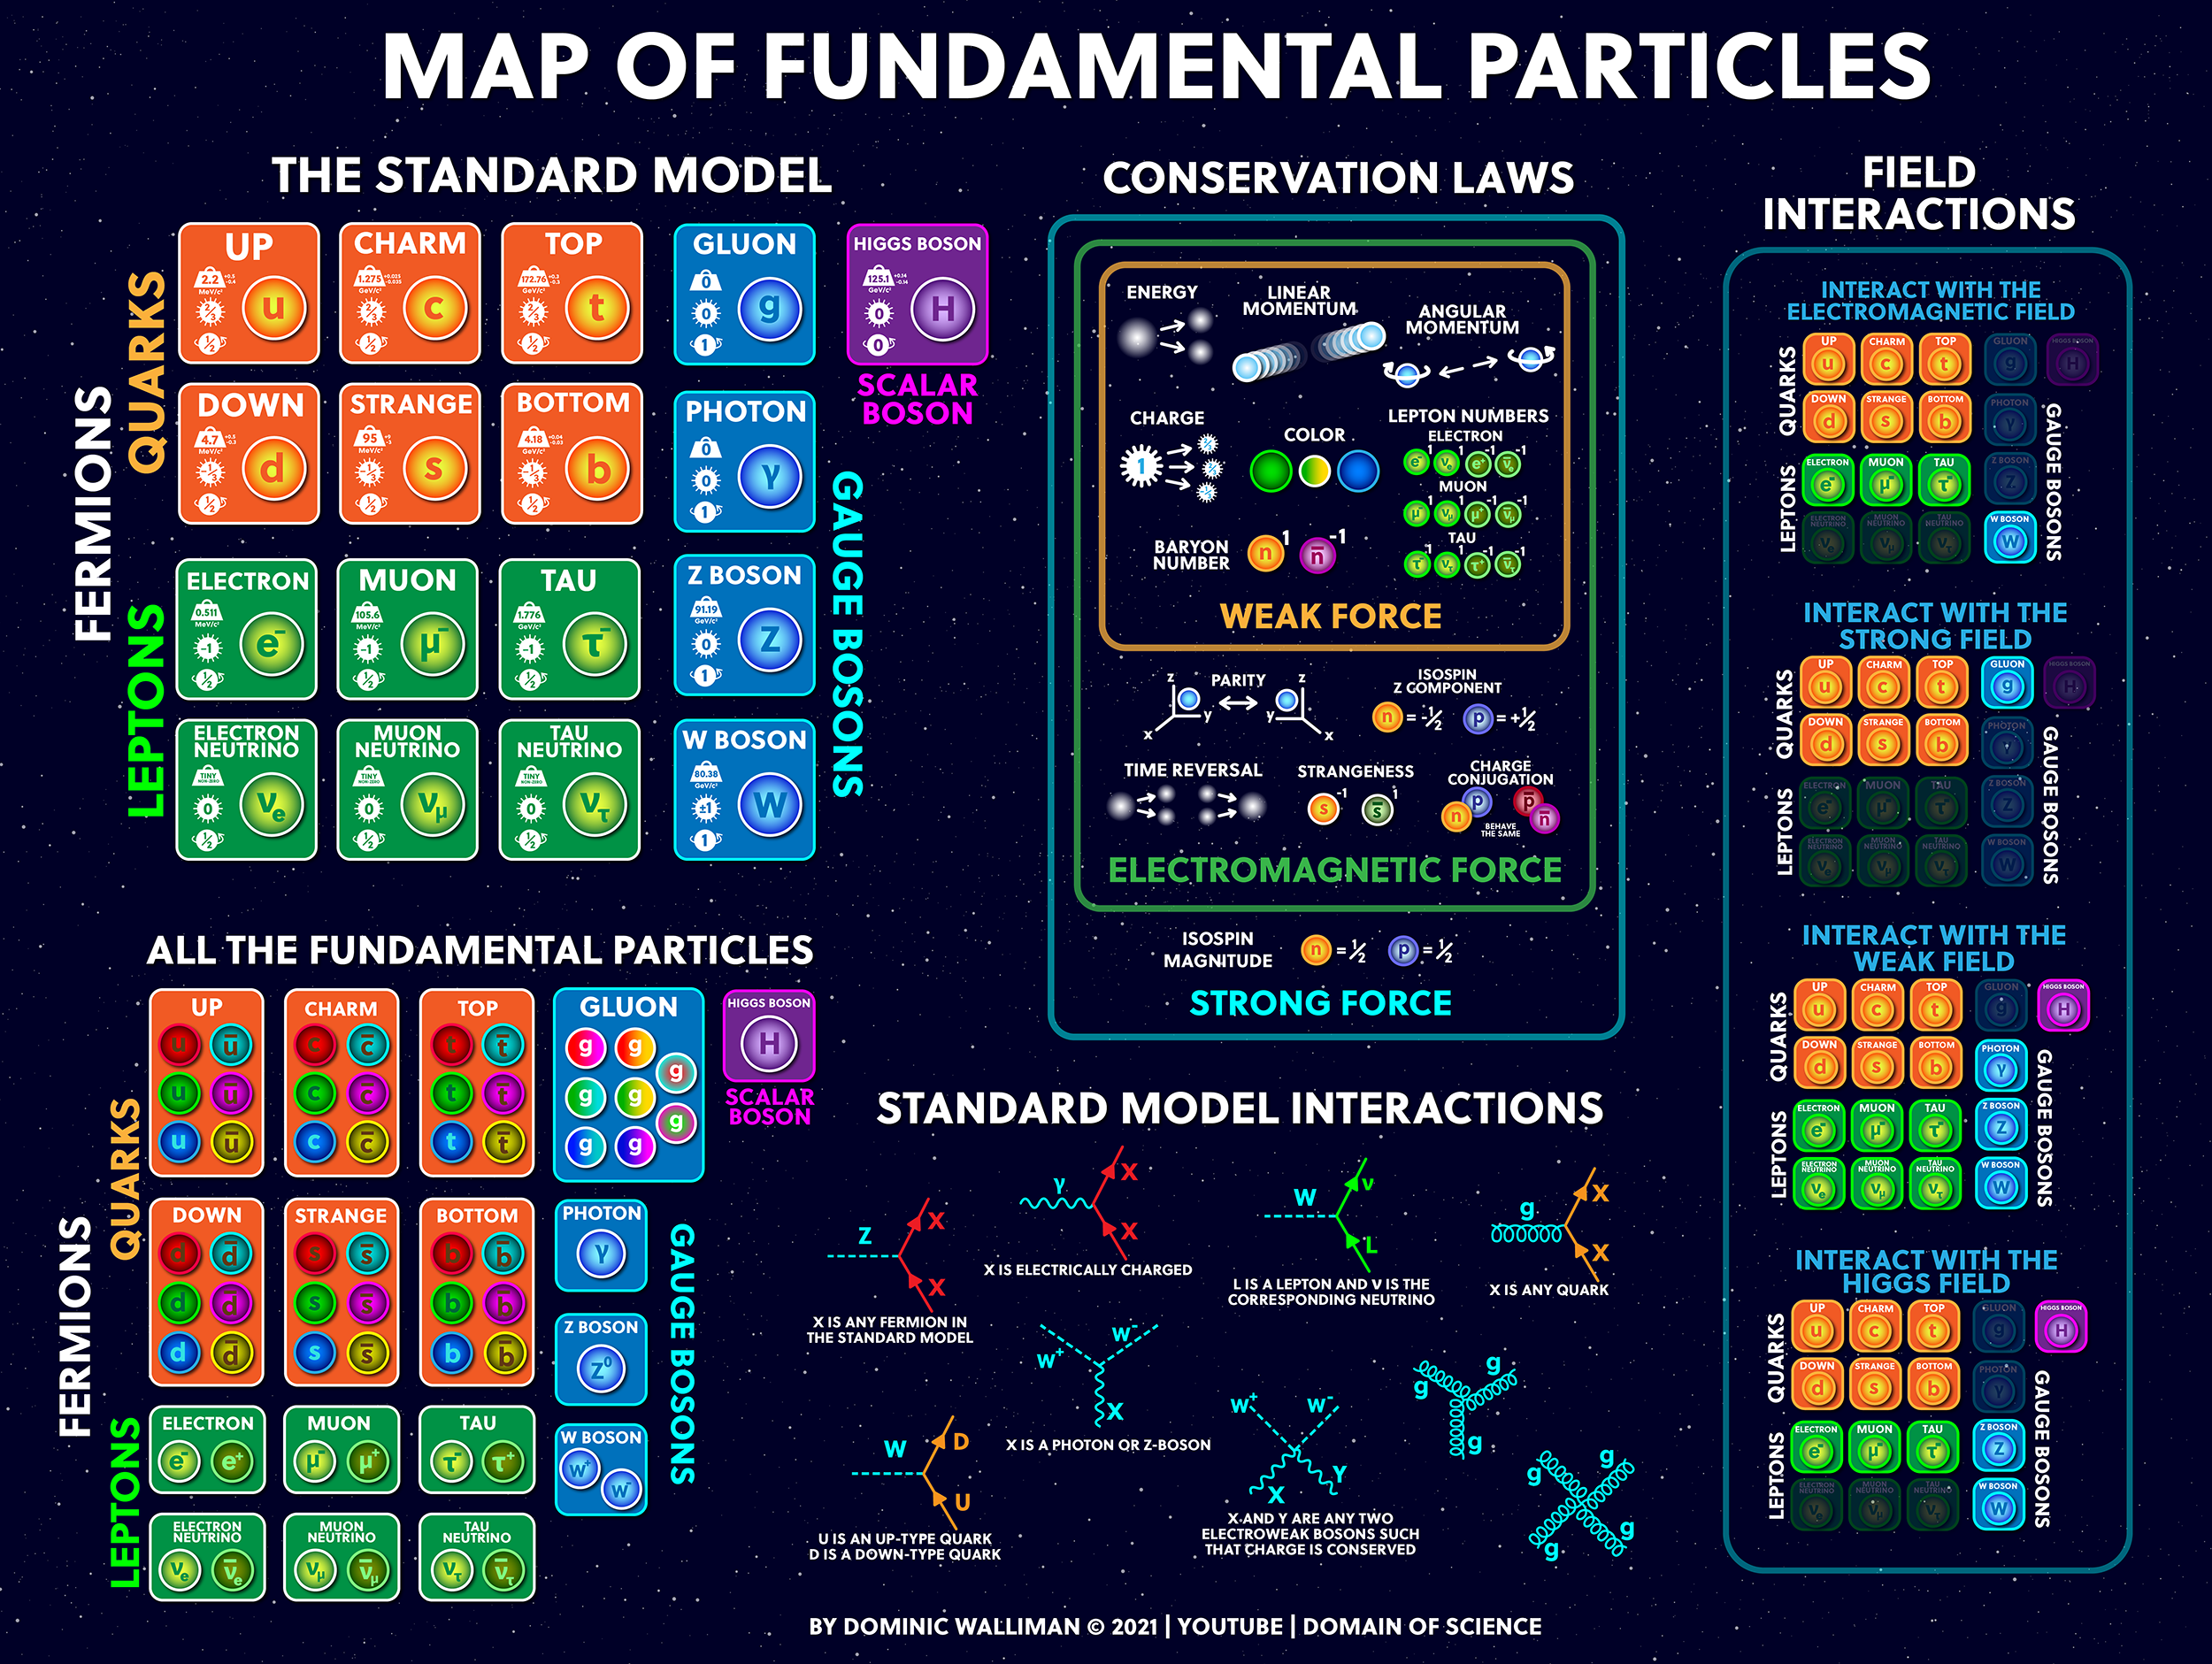
\includegraphics[width=1.5\linewidth]{Billeder/Cheat.png}}
    \label{fig:Cheat}
\end{figure}

\section{Units}
To simplify calculations we switch to natrual units, 
where $c = \h = 1, k=1/4\pi$, and therefore all units are in powers of eV.
We can then say that 
\begin{align*}
    (NU) = \h^ac^b(SI)
\end{align*}
and with that go between systems. Some good conversions to remember is: 
\begin{align*}
    &\h c \approx \SI{197}{MeV.fm}, \eq{1.17}\\
    &\h \approx \SI{6.58e{-16}}{eV.s} \eq{1.18}.
\end{align*}

\chapter{Scattering and Decay}
\section{Special Relativity}
Covariance is a prescription on the form of the physical laws
that ensures compliance with the axioms of relativity:

(A1) The physical laws retain the same functional form in all
inertial frames.

(A2) The speed of light in vacuum is the same for all inertial
observers.

The Four-vector for location is 
\begin{align*}
    x^μ = (ct, x, y, z) \eq{2.19},
\end{align*}
and the transformed vector is:
\begin{align*}
    \mat{x_0'\\ x_1'\\ x_2'\\ x_3'} =
    \begin{pmatrix}
        γ & βγ & 0 & 0 \\
        βγ & γ & 0 & 0 \\
        0 & 0 & 1 & 0 \\
        0 & 0 & 0 & 1
    \end{pmatrix}
    \mat{x_0\\ x_1\\ x_2\\ x_3}, \eq{2.21}
\end{align*}
\begin{align*}
    x'^μ=Λ^μ_ν x^ν. \eq{2.22}
\end{align*}

The velocity and acceleration four vectors are: 
\begin{align*}
    v^μ &= γ(c, v_x, v_y, v_z), \\
    a^μ &= γ(\dot{γ}c, \dot{γ}\v{v}+γ\v{a}). 
\end{align*}

The four-momentum is: 
\begin{align*}
    p^μ = (mγ, mγ\v{v}) = (E, \v{p}), \eq{2.40}
\end{align*}
We can use this to calcualte energies in particle interactions, 
since we know there is conservation of momentum. 
\begin{align*}
    \sum_{i=1}^{N_i}p^μ_i = \sum_{j=1}^{N_f}p^μ_j. \eq{2.43}
\end{align*}
Some helpful equations are: 
\begin{align*}
    & (p^μ)^2 = (p^0)^2-|\v{p}|^2, \eq{2.57}\\
    & E = p^0 = (m^2+|\v{p}|^2)^{1/2}. \eq{2.58}
\end{align*}

\section{Two-body decay}
Creation or destruction of particles can only happen if kinematics of Special relativity and of laws of the standard model are conserved. 
For decays of one particle $a$ into two particles, the momentum must be conserved: 
\begin{align*}
  p_a^μ = p_1^μ+p_2^μ \eq{2.64}, 
\end{align*}
if we look at the rest frame of $a$, we get that 
\begin{align*}
  p_2^2=\br{p_a-p_1}^2=p_a^2+p_1^2-2 p_a\cdot p_1, \eq{2.65} \\
  m_2^2=m_a^2+m_2^2-2 p_a^μ\cdot p_{1μ}. \eq{2.66}
\end{align*}
Here we used that the norm of a single particles momentum is it's rest mass. 
Because we are in the rest frame of $a$
\begin{align*}
  p_a^μp_{1μ} = g_{μν}p_a^μp_1^ν=m_aE_1 \eq{2.67},
\end{align*}
and with this we have: 
\begin{align*}
  E_1 = \frac{m_a^2+m_1^2-m_2^2}{2m_a}, \quad E_2 = \frac{m_a^2+m_2^2-m_1^2}{2m_a}. \eq{2.68}
\end{align*}

\subsection{Three-body decay}
In a three-body decay $a \rightarrow 1+2+3$, we have too many variables, and can therefore only say something about the 
minimum and maximum energy of particle $1$. 
\begin{align*}
  m_1 \leq E_1^{CM}\leq \frac{m_a^2+m_1^2-(m_2+m_3^2)}{2m_a}. \eq{2.71}
\end{align*}

\section{Decay Amplitudes}
In a general term we can use the \textbf{relativistic golden rule} for unstable particles that decay into $N_f$ particles. 
We use this rule to calcualte the transition rate, which is the probability per unit time that the particle in the initial state decay into the final state:
\begin{align*}
  Γ_{i\rightarrow f} = \frac{1}{2E_a}\int\prod_{i=1}^{N_f}\frac{d^4p_i}{(2\pi)^4}\br[5]{\mathscr{M}}^2(2\pi)^4δ^4\br{p_a-\sum_{j=1}^{N_f}p_j} \times (2\pi) δ\br{p_i^2-m_i^2}. \eq{2.90}
\end{align*}

The decay Lorentz transforms as 
\begin{align*}
  Γ'_{i\rightarrow f} = Γ_{i\rightarrow f} / γ. \eq{2.94}
\end{align*}
And is ralated to the lifetime of a particle by 
\begin{align*}
  τ = 1/Γ. \eq{2.96}
\end{align*}
But most particles decay in multiple nodes and we therefore have to generalize as: 
\begin{align*}
  τ = \frac{1}{Γ} = \frac{1}{\sum_{i=1}^{N}Γ_i}. \eq{2.101}
\end{align*}
The \textbf{Branching Ratio} of node $i$ is defined as: 
\begin{align*}
  \text{BR}(i) = \frac{Γ_i}{Γ}. \eq{2.102}
\end{align*}

In (2.90) we have $\M$ which is the Lorentz-invarient matrix element for n-body decay: 
\begin{align*}
  \mathscr{M} = (2E_a)^{1/2}\prod_{i=1}^{N_f}(2E_i)^{1/2}\mathscr{T}, \eq{2.79}
\end{align*}
where $\mathscr{T} = \hv[f]{}\hat{H}\hv{i}$


\section{Scattering}
Most of the formulas for decay holds for two-body scattering $a+b \rightarrow 1+...+n$, we just have to make a few corrections. 
A measurement for scattering in QM is the \textbf{differential cross section}, which is the ratio between the number of particles 
that are scattered in a solid angle between $Ω$ and $Ω+dΩ$ per unit time divided by the flux (the rate of incomming particles per unit surface). 
Or in other words the likelihood that a particle is scattered at an angle $Ω$. 
\begin{align*}
  \frac{dσ}{dΩ}(E, Ω) = \frac{1}{F}\frac{dN_s}{dΩ}. \eq{2.113}
\end{align*} 

This leads to the \textbf{relativistic golden rule for the cross section} 
\begin{align*}
  \sigma_{i \to f} &= \frac{(2\pi)^4}{2E_a 2E_b |v_a - v_b|} \int \prod_{i=1}^{n} \frac{d^3\v{p}_i}{(2\pi)^3 2E_i} \\ 
  &\times |\mathcal{M}|^2 \delta\left(E_a + E_b - \sum_{j=1}^{n} E_j\right) \delta^3\left(\v{p}_a + \v{p}_b - \sum_{j=1}^{n} \v{p}_j\right), \eq{2.128}
\end{align*}
but here we have a new $\mathscr{M}$
\begin{align*}
  \mathscr{M} = (2E_a)^{1/2}(2E_b)^{1/2}\prod_{i=1}^{n}(2E_i)^{1/2}\mathscr{T}. \eq{2.127}
\end{align*}

A usefull Lorentz-invarient is the \textbf{first Mandelstam variable} for two-body scattering 
\begin{align*}
  s = (p_a+p_b)^2 =(p_{tot})_μ(p_{tot})^μ \eq{2.131},
\end{align*}
where $(p_{tot})^μ=p_a^μ+p_b^μ$ is the total initial momentum. $\sqrt{s}$ is often called invarient mass. 
The goal of QFT is to calculate $\mathscr{M}$ and in most cases $\br[5]{\mathscr{M}}^2$ is a smooth and slowly variable function of $s$.
If $\br[5]{\mathscr{M}}^2 \approx$ constant then 
\begin{align*}
  σ = \frac{1}{s}, \eq{2.136}
\end{align*} 
for $\sqrt{s} \gg m_a, m_b$. 

\setcounter{chapter}{4}
\chapter{Symmetries}
\section{Symmetries in Quantum Mechanics }
In quantum mechanics (QM), a symmetry is a set of transformations represented by \textbf{unitary} (or anti-unitary) \textbf{operators}, $U$, that leave physical observables unchanged. 
This requires $U^\dagger U = \text{I}$. A system's Hamiltonian, $H$, is invariant under a symmetry transformation if it commutes with the symmetry operator, $[H, U] = 0$. 
\textbf{Wigner's theorem} states that all symmetries in QM are represented by such unitary or anti-unitary operators that commute with the Hamiltonian. 
If $[H, U] = 0$, the expectation value $\langle U \rangle$ is constant in time, making it an integral of motion, though not necessarily a directly measurable conserved physical quantity since $U$ may not be Hermitian.

\section{Classification of Symmetries}
Symmetries in QM can be \textbf{classified} into four types:
\begin{itemize}
    \item \textbf{Continuous external:} Depend smoothly on parameters and change space-time coordinates (e.g., translations, rotations).
    \item \textbf{Continuous internal:} Depend smoothly on parameters but \emph{do not} change space-time coordinates.
    \item \textbf{Discrete external:} Involve a finite set of transformations that change space-time coordinates (e.g., parity $P$).
    \item \textbf{Discrete internal:} Involve a finite set of transformations that \emph{do not} change space-time coordinates (e.g., charge conjugation $C$).
\end{itemize}
\textbf{Continuous symmetries} described by unitary operators $U(a_j)$ can be expressed exponentially in terms of \textbf{Hermitian generators} 
\begin{align*}
  T_j: U(a_1...a_N) = e^{i\sum_j a_j T_j}. \eq{5.9}
\end{align*}
Because these generators $T_j$ are Hermitian and commute with the Hamiltonian $H$, their expectation values $\langle T_j \rangle$ represent \textbf{conserved physical quantities}.

\section{Inversion}
Inversions are discrete transformations, the unitary operator has to fulfill 
\begin{align*}
  U^2=\text{I}, \eq{5.26}
\end{align*}
and if the operator is applied twice we should return to the original system. 
One such symmetry could be \textbf{parity} where we invert $\v{x}$ turning a right hand system to a left hand system. 
\begin{align*}
  \mathcal{P}\hv{x} = \hv{-x}, \eq{5.27}
\end{align*}
which in quantum mechanics is a unitary, hermitian operator 
\begin{align*}
  \mathcal{P}ψ(\v{x}) = ψ(-\v{x}). \eq{5.28}
\end{align*}
The parity of a system is only defined if the wavefunction is an eigenstate of $\mathcal{P}$, 
with eigenvalues $+1$ (even parity) or $-1$ (odd parity).

\section{The Intrinsic Parity of Particles}
In QM we define the \textbf{intrinsic parity} of a particle, as the eigenvalue of the wavefunction of the particle in its restframe. 
For a photon we can not find the intrinsic parity directly with QM, so we look at the decay of exited hydrogen: 
\begin{align*}
  \atom{H}{1}{1}^{*} \rightarrow \atom{H}{1}{1} + γ \eq{5.34},
\end{align*}
We know that the parity of hydrogen is 
\begin{align*}
  \mathcal{P}ψ_{H} = (-1)^lψ_{H}, \eq{5.40}
\end{align*}
we can extend this to our decay 
\begin{align*}
  \mathcal{P}ψ_{H}ψ_γ = (-1)^{l_{fin}} ψ_{H} \mathcal{P}_γψ_γ, \eq{5.41}
\end{align*}
where $l_{fin}$ is the angular momentum number in the final state of H, and $\mathcal{P}_γ$ is the intrinsic parity of the photon. 
In the initial state we have $\mathcal{P}ψ_{H^*} = (-1)^{l_{in}}ψ_{H^*}$, and we know that the electric dipole transition happends at $Δl= \pm 1$, 
therefore the intrinsic parity of the photon is $-1$ if partity is conserved in electromagnetic ineractions. 

The intrinsic parity of all negatively charged elementary leptons and all neutrinos is $+1$, 
as well as all quarks. For antifermions the intrinsic parity is opposide the corresponding fermion, but for antobosons it is the same as the corresponding boson. 
If we exchange a pair of fermions the spin part of the wavefunction changes as $(-1)^{1+s}$, and if we exchange a pair of bosons it changes as $(-1)^s$. 

\section{C-Parity}
A C-parity transform a particle into its antiparticle (inverts charge). 
For classical mechanics this means changing both the sign of electric and magnetic fields, this gives us that the C-parity of a photon is $-1$. 
It is only neutral particles that can be eigenstates of the C-parity operator, meaning they are their own antiparticle. 
For neutrinos we dont know if they are thier own antiparticle. 

\subsection{Particle-Antiparticle Pairs}
For particle-antiparticle pairs we know that the C-parity of a boson-antiboson is $+1$ and for a fermion-antifermion pair it is $-1$. 
If the two particles have no spin the C-operator is the same as the parity-operator 
\begin{align*}
  Cψ = Pψ = (-1)^lψ. 
\end{align*}
If they have spin the C-parity operator is the exchange of the two particles 
\begin{align*}
  Cψ = (-1)^{l+s}ψ. \eq{5.66}
\end{align*}

\section{T-Parity and CPT}
T-parity is flipping the time axis. This symmetry is conserved in strong and QED interaction, but not always in weak interactions. 
This means that a motion in time, is also allowed reversed in time and happens at the same rate. 
A system is not nessecarily invarient to any of the operators when applied individually, 
but if we apply all three parity operators $(\mathcal{CPT})$, the system will be invarient, 
"it is a symmetry in any Lorentz invarient local quantum field theory with hermitian Hamiltonian." 

\section{The Dirac Equation}
The Dirac equation is used to describe the wavefunction, of spin-1/2 particles with mass $m$, in space-time: 
\begin{align*}
  \br{iγ^μ\partial_μ-m}ψ(x^μ)=0. \eq{5.82}
\end{align*}
It introduces the bispinor wanvefunction $ψ(x^μ)$, which is a vector of 4 wavefuntions, and the Dirac matrices: 
\begin{align*}
\gamma^0 &= \begin{pmatrix} 1 & 0 & 0 & 0 \\ 0 & 1 & 0 & 0 \\ 0 & 0 & -1 & 0 \\ 0 & 0 & 0 & -1 \end{pmatrix} &
\gamma^1 &= \begin{pmatrix} 0 & 0 & 0 & 1 \\ 0 & 0 & 1 & 0 \\ 0 & -1 & 0 & 0 \\ -1 & 0 & 0 & 0 \end{pmatrix} \\
\gamma^2 &= \begin{pmatrix} 0 & 0 & 0 & -i \\ 0 & 0 & i & 0 \\ 0 & i & 0 & 0 \\ -i & 0 & 0 & 0 \end{pmatrix} &
\gamma^3 &= \begin{pmatrix} 0 & 0 & 1 & 0 \\ 0 & 0 & 0 & -1 \\ -1 & 0 & 0 & 0 \\ 0 & 1 & 0 & 0 \end{pmatrix}. \eq{5.81}
\end{align*}

The solution the the Dirac equation can be spilt into two; the postive energy solution and the negative energy solution. 
These solution (eq 5.85 and 5.86) show that 
"if a particle satisfies the Dirac equation, it is a spin-1/2 fermion and its intrinsic magnetic moment is proportional to the spin $\mathbf{S}$. "

\chapter{Electromagnetic Interactions}
Read Elyn Notes $:($

\chapter{Strong Interactions}
Quarks interact with the strong force using gluons, which are simmilar to photons. 
They do this through the color charge of the quarks. A quark can either $+1$ blue, red or green charge, 
and an anti quark can have $-1$ blue, red or green charge. 
Quarks and antiquarks also have electrical charges, which can be seen in the fundamental map. 
A hadron then has the sum of all the charges of its quarks. 


\chapter{Flavour and Quark Model}
\section{Baryons in the Two/Three-quark Model}
Chapter 8 goes through the total wavefunction of quarks, and how they interact in a baryon. 
There is a little about group theory, but not really how to calculate it. 
For the two-quark model, that is where we only use up and down, the total wavefunction for a baryon is 
\begin{align*}
  Ψ = ψ_{space}ψ_{spin}ψ_{color}ψ_{flavor}. \eq{8.16}
\end{align*}
The total wavefunction for a baryon has to be anti-symmetric, according to Pauli exclusion principle. 
The spin wavefunction is anti-symmetric and the space wavefunction is symmetric, so the color and flavor wavfunctions has to be symmetric.

If we extend to the three-quark model where we include the strange quark, the $ψ_{space}ψ_{color}$ wavefunction is antisymmetric, 
and the spin wave function has to be $ψ_{spin}^{S=3/2}$. 

\section{Isospin}
Up type quarks have isospin $I_z=+1/2$ and down has $I_z=-1/2$. And anti particles have different sign. 
Isospin has nothing to do with the angular momentum of the particles, as all quarks are spin-1/2 particles. 
So when building Hadrons we can have total isospin, which is then a measure of if the hadron is down or up. 
If we put this on the x-axis, and then the flavours on the y-axis we can create isospin plots like shown in fig \ref{fig:Iso}
\bil{Iso}

\section{Mesons in the Two/Three-quark Model}
For mesons we do not require the wavefunction to be anti-symmetric. The parity and C-parity of a meson is 
\begin{align*}
  Pψ = Cψ = (-1)^{l+s} \eq{8.43}.
\end{align*}

\section{Generalization of the Quark Model}
We introduce a new quantum number called the baryon number which is $+1/3$ for quarks, and $-1/3$ for anti-quarks. 
This number must be conserved in all interactions. 
For the modern classification we use the five-quark model which approximates that all quarks exept top has the same mass. 
Top has a much higher mass, and decays before it can be bound in a hadron. 
Tetraquarks and Pentaquarks are possible but it is hard to distinguish them from a meson-meson binding and baryon-meson binding. 


\chapter{From QCD to Nuclear}
\setcounter{section}{3}
\section{Nuclear Shell Model}
\subsection{Universal Filling order}
\begin{itemize}
  \item $1s_{1/2} (2) \quad \rightarrow \mathbf{2}$
  \item $1p_{3/2} (4) \quad 1p_{1/2} (2) \quad \rightarrow \mathbf{8}$
  \item $1d_{5/2} (6) \quad 2s_{1/2} (2) \quad 1d_{3/2} (4) \quad \rightarrow \mathbf{2 0}$
  \item $1f_{7/2} (8) \quad \rightarrow \mathbf{2 8} $
  \item $2p_{3/2} (4) \quad 1f_{5/2} (6) \quad 2p_{1/2} (2) \quad 1g_{9/2} (10) \quad \rightarrow \mathbf{5 0}$
  \item $1g_{7/2} (8) \quad 2d_{5/2} (6) \quad 3s_{1/2} (2) \quad 1h_{11/2} (12) \quad 2d_{3/2} (4) \quad \rightarrow \mathbf{8 2}$
  \item $ 2f_{7/2} (8) \quad 1h_{9/2} (10) \quad 3p_{3/2} (4) \quad 2f_{5/2} (6) \quad 3p_{1/2} (2) \quad 1i_{13/2} (14) \quad \rightarrow \mathbf{1 2 6}$
  \item $2g_{9/2} (10) \quad 1i_{11/2} (12) \quad 1j_{15/2} (16) \quad 3d_{5/2} (6) \quad 2g_{7/2} (8) \quad 4s_{1/2} (2) \quad 3d_{3/2} (4) \quad \rightarrow \mathbf{1 8 4}$
\end{itemize}

\subsection{Determining Nucleus Spin and Parity}
\begin{itemize}
  \item Check Number of Protons (Z) and Neutrons (N):
  \begin{itemize}
    \item If both are even, the ground state has $I=0$ and parity $+$. 
    \item If one is odd the spin is determined by the valence nucleon. 
    \item If both are odd the spin is detemined both by the spin of the unpaired proton and nucleon. 
  \end{itemize}
  If A is odd fill the shells with the number of nucleons in accordance with figure \ref{fig:Shell}.
  From that we then know $I=i$ and $P=(-1)^l$. 

  If both are odd do this for both and then 
  \begin{align*}
    P &= P_p \times P_n \\
    |i_p-i_n| &\leq I \leq i_p + i_n
  \end{align*}
\end{itemize}
\bil{Shell}

\section{Magnetic Moment}
This is not in the book but used for exercise 1 in 2023. 
The magnetic moment of a nucleus is decided from the valence particle, and calculated as
\begin{align*}
  μ_j = \br{g^{(l)}l+\frac{1}{2}g^{(s)}}μ_N, \quad \text{ if } j=l+1/2, \\
  μ_j = \frac{j}{j+1}\br{g^{(l)}(l+1)-\frac{1}{2}g^{(s)}}μ_N, \quad \text{ if } j=l-1/2,
\end{align*}
where $μ_N$ is the nuclear magneton, and for a neutron $g^{(l)}=0$, $g^{(s)}=-3.8263$ and for a proton $g^{(l)}=1$, $g^{(s)}=5.5858$. 

\setcounter{chapter}{10}
\chapter{Radioactivity}
\setcounter{section}{3}
\section{Beta Decay Selection Rules}
Allowed beta decays are $ΔI=0$ which are Fermi decays, 
if the total spin does not go from 0 to 0 and there is no parity change, 
then it is also a Gamov-Teller decay. 



\newpage
\chapter{Appendix}
\section{Four-Vector}
A four-vector $a^\mu$ is an object in Minkowski space-time with four components. It is written as:
\[
a^\mu = (a^0, a^1, a^2, a^3) = (a^0, \mathbf{a})
\]
where $a^0$ is the time-like component and $\mathbf{a} = (a^1, a^2, a^3)$ is the vector of the space-like components.

\subsection{Contravariant and Covariant Vectors}
A four-vector can be in two forms:
\begin{itemize}
    \item \textbf{Contravariant} (upper index): $a^\mu = (a^0, a^1, a^2, a^3)$
    \item \textbf{Covariant} (lower index): $a_\mu = (a_0, a_1, a_2, a_3)$
\end{itemize}
The transformation between them uses the Minkowski metric tensor $g_{\mu\nu}$.
\begin{equation}
g_{\mu\nu} = \begin{pmatrix} 1 & 0 & 0 & 0 \\ 0 & -1 & 0 & 0 \\ 0 & 0 & -1 & 0 \\ 0 & 0 & 0 & -1 \end{pmatrix} \label{eq:metric} \tag{2.31}
\end{equation}
The rule to lower an index is $a_\mu = g_{\mu\nu}a^\nu$. This results in:
\[
a_\mu = (a^0, -a^1, -a^2, -a^3) = (a^0, -\mathbf{a})
\]

\subsection{Scalar Product}
The scalar product of two four-vectors $a^\mu$ and $b^\mu$ is a Lorentz invariant scalar, denoted as $a \cdot b$ or $a_\mu b^\mu$.
\begin{equation}
a \cdot b = a_\mu b^\mu = g_{\mu\nu} a^\mu b^\nu \label{eq:scalarprod}
\end{equation}
Using the Einstein summation convention, this expands to:
\[
a \cdot b = a^0 b^0 - a^1 b^1 - a^2 b^2 - a^3 b^3 = a^0 b^0 - \mathbf{a} \cdot \mathbf{b}
\]

\subsection{Squared Norm of a Four-Vector}
The squared norm of a four-vector $a^\mu$ is its scalar product with itself, denoted $a^2$.
\begin{equation}
a^2 = a_\mu a^\mu = (a^0)^2 - (a^1)^2 - (a^2)^2 - (a^3)^2 = (a^0)^2 - |\mathbf{a}|^2 \label{eq:norm}
\end{equation}
The sign of the squared norm classifies the four-vector:
\begin{itemize}
    \item $a^2 > 0$: \textbf{Time-like}
    \item $a^2 < 0$: \textbf{Space-like}
    \item $a^2 = 0$: \textbf{Light-like} or \textbf{null}
\end{itemize}

\subsection{The Four-Momentum}
The four-momentum $p^\mu$ is a key four-vector in relativistic kinematics. In natural units ($c=1$), it is defined as:
\begin{equation}
p^\mu = (E, \mathbf{p}) = (m\gamma, m\gamma\mathbf{v}) \label{eq:4momentum} \tag{2.40}
\end{equation}
where $E = m\gamma$ is the relativistic energy, $\mathbf{p} = m\gamma\mathbf{v}$ is the relativistic three-momentum, $m$ is the rest mass, and $\gamma = 1/\sqrt{1 - v^2}$ is the Lorentz factor.

The squared norm of the four-momentum is the squared rest mass, an invariant:
\[
p^2 = p_\mu p^\mu = E^2 - |\mathbf{p}|^2 = m^2
\]
This yields the energy-momentum relation:
\begin{equation}
E = \sqrt{|\mathbf{p}|^2 + m^2} \label{eq:emrelation} \tag{2.58}
\end{equation}

\subsection{Lorentz Transformations}
A four-vector $a^\mu$ transforms between inertial frames via a Lorentz transformation matrix $\Lambda^\mu_\nu$.
\[
a'^\mu = \Lambda^\mu_\nu a^\nu
\]
For a boost with velocity $v$ along the $x^1$-axis, the matrix is:
\[
\Lambda^\mu_\nu = \begin{pmatrix} \gamma & -\beta\gamma & 0 & 0 \\ -\beta\gamma & \gamma & 0 & 0 \\ 0 & 0 & 1 & 0 \\ 0 & 0 & 0 & 1 \end{pmatrix}
\]
where $\beta = v$ in natural units. Applying this to the four-momentum $p^\mu=(E, p_x, p_y, p_z)$ gives:
\begin{align*}
E' &= \gamma(E - \beta p_x) \\
p'_x &= \gamma(p_x - \beta E) \\
p'_y &= p_y \\
p'_z &= p_z
\end{align*}

\end{document} % ----------Dokumentet er nu slut! ------------